\section{Resultados preliminares de topología general}

\subsection{Espacios topológicos y continuidad}

\begin{definicion}{Topología}{def_topologia}
Sea $X$ un conjunto. Recordemos que una topología en $X$ es una familia $\tau \subseteq \mathcal{P}(X)$ tal que:
\begin{enumerate}
    \item $\emptyset$ y $X$ están en $\tau$.
    \item La unión de los elementos de cualquier subcolección de $\tau$ está en $\tau$.
    \item La intersección de los elementos de cualquier subcolección finita de $\tau$ está en $\tau$.
\end{enumerate}
\end{definicion}

\begin{nota}{Espacios métricos}{nota_metricos}
Todo espacio métrico $(X, d)$ es un espacio topológico:
\[ \tau = \{A \subseteq X \mid \text{para todo } x \in A, \exists \varepsilon > 0 \text{ tal que } B(x, \varepsilon) \subseteq A\} \]
\end{nota}

\begin{definicion}{Topología de subespacio}{def_subespacio}
Sea $X$ un espacio topológico. Sea $B \subseteq X$. La topología en $B$ inducida por la de $X$ es:
\[ \tau_B = \{A \cap B \mid A \text{ es abierta en } X\} \]
Se le llama topología de subespacio o heredada por la de $X$.
\end{definicion}

\begin{definicion}{Continuidad}{def_continua}
Sea $f \colon X \to Y$ una aplicación (suponemos $X, Y$ espacios topológicos). Se dice que $f$ es continua cuando:
\[ \forall A \in \tau_Y, \quad f^{-1}(A) \in \tau_X \]
Es decir, la antiimagen de todo abierto en $Y$ es un abierto en $X$.
\end{definicion}

\subsection{Homeomorfismos e invariantes topológicos}

\begin{definicion}{Homeomorfismo}{def_homeomorfismo}
Sea $f \colon X \to Y$ una aplicación. Se dice que $f$ es un homeomorfismo cuando:
\begin{itemize}
    \item $f$ es continua.
    \item $f$ es biyectiva.
    \item $f^{-1}$ es continua.
\end{itemize}
\end{definicion}

\begin{nota}{Noción de isomorfismo}{nota_isomorfismo}
En matemáticas se suele tener una noción sobre qué es que dos cosas sean lo mismo. Por ejemplo, sea $f \colon G_1 \to G_2$ una aplicación donde $G_1, G_2$ son grupos. Se dice que $f$ es un isomorfismo de grupos si $f$ es un homomorfismo y $f$ es biyectiva.
\end{nota}

\begin{observacion}{Equivalencia topológica}{obs_equivalencia}
La \cref{def_homeomorfismo} es la noción natural de equivalencia en la categoría de espacios topológicos, es una forma de establecer el significado de cuándo dos espacios son lo mismo.
\end{observacion}

Sean $X, Y$ espacios topológicos. Diremos que $X$ e $Y$ son homeomorfos si $\exists f \colon X \to Y$ homeomorfismo. Esta definición es análoga a la de isomorfismo de grupos: se dice que $G_1, G_2$ son grupos isomorfos cuando $\exists f \colon G_1 \to G_2$ isomorfismo. De igual forma, espacios $E_1, E_2$ son espacios isomorfos.

\textbf{Pregunta natural:} Dados $X, Y$ espacios topológicos, ¿existe forma/algoritmo para decidir si $X$ e $Y$ son homeomorfos?

\begin{enumerate}
    \item Si $X = [0,1]$, es compacto. Si $Y = \left]0,1\right[$, no es compacto. (Suponemos la topología usual). $\implies$ No son homeomorfos. $X \not\cong Y$.
    \item Si $X = [0,1]$ (no finito) y $Y = \{0,1\}$ (finito) $\implies X \not\cong Y$. No son homeomorfos.
    \item Si $X = [0,1] \setminus \{1/2\}$, entonces $X$ no es conexo. Si $Y = [0,1]$, $Y$ es conexo. $\implies X \not\cong Y$ por invariante topológico.
    \item $X = [0,1]$ y $Y = \{z \in \mathbb{C} \mid |z| = 1\} = S^1$.
    \textbf{Spoiler:} Asociamos a un espacio un Grupo Fundamental: $X \rightsquigarrow \pi_1(X)$. Si dos espacios son homeomorfos, entonces sus grupos fundamentales son isomorfos ($X \cong Y \implies \pi_1(X) \cong \pi_1(Y)$). No es un invariante topológico completo. Veremos más adelante con la noción de grupo fundamental que $X$ e $Y$ no son homeomorfos.
    \item Sea $S^2 \subseteq \mathbb{R}^3$, donde $S^2 = \{(x,y,z) \in \mathbb{R}^3 \mid ||(x,y,z)|| = 1\} \implies$ Grupo trivial.
    
    \begin{center}
    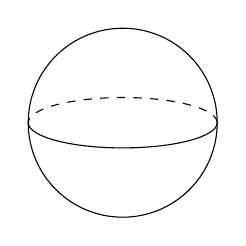
\begin{tikzpicture}[scale=0.8]
      \draw (0,0) circle (1.5cm);
      \draw[dashed] (1.5,0) arc (0:180:1.5 and 0.4);
      \draw (1.5,0) arc (0:-180:1.5 and 0.4);
    \end{tikzpicture}
    \end{center}
    
    Sea $T^2 \subseteq \mathbb{R}^3$, donde $T^2 \cong S^1 \times S^1 \subseteq \mathbb{R}^4 \implies$ Grupo $\mathbb{Z} \times \mathbb{Z}$.
    
    \begin{center}
    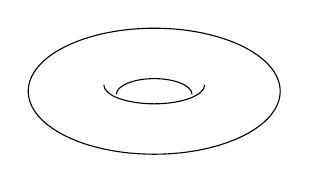
\begin{tikzpicture}[scale=0.8]
      \draw (0,0) ellipse (2 and 1);
      \draw (-0.8,0.1) arc (180:360:0.8 and 0.3);
      \draw (-0.6,-0.05) arc (180:0:0.6 and 0.25);
    \end{tikzpicture}
    \end{center}
    
    Sus grupos fundamentales no son isomorfos, luego $S^2 \not\cong T^2$.
\end{enumerate}

\begin{observacion}{Sobre el ejemplo 4}{obs_ejemplo4}
A pesar de que más adelante aplicaremos la noción de grupo fundamental para deducir que no son homeomorfos, encontraremos otra vía más sencilla para concluir que no son homeomorfos.
\end{observacion}

\begin{definicion}{Invariante por componentes conexas}{def_componentes}
Sea $X$ un espacio topológico. Sea $p \in X$. Denotamos por $C_p(X)$ el nº de componentes conexas de $X \setminus \{p\}$.
\end{definicion}

Es muy sencillo probar que $\{C_p(X) \mid p \in X\} := \Theta(X)$ es un invariante topológico de $X$ (Ejercicio).
\[ X \cong Y \implies \Theta(X) = \Theta(Y) \]

\textbf{Ejemplos:}
\begin{itemize}
    \item Cruz: $C_{(0,0)}(X) = 4$, $C_{(1/2,0)}(X) = 2$. $\Theta(X) = \{1,2,4\}$.
    
    \begin{center}
    \begin{tikzpicture}[scale=1]
      \draw[thick] (-1.5,0) -- (1.5,0);
      \draw[thick] (0,-1.5) -- (0,1.5);
      \node[anchor=north east] at (0,0) {$0$};
      \node[anchor=north] at (1.5,0) {$1$};
      \node[anchor=north] at (-1.5,0) {$-1$};
      \node[anchor=east] at (0,1.5) {$1$};
      \node[anchor=east] at (0,-1.5) {$-1$};
    \end{tikzpicture}
    \end{center}
    
    \item Línea $Y$: $\Theta(Y) = \{1,2,3\}$.
\end{itemize}

\subsection{Conexión y Compacidad}

\begin{definicion}{Desconexión y conexión}{def_desconexion}
Sea $X$ un espacio topológico. Una desconexión de $X$ es el par $(A,B)$ de abiertos de $X$ tal que $A \cup B = X$, $A, B \neq \emptyset$, $A \cap B = \emptyset$.
Diremos que $X$ es conexo cuando no admite ninguna desconexión.
Diremos que $X$ es disconexo cuando no es conexo, es decir, cuando admite una desconexión.
\end{definicion}

\textbf{Ejemplo:} $[0,1]$ es conexo. $B = [0,1] \cup [2,15]$ es disconexo. Insistimos en que en los ejemplos, cuando consideramos subconjuntos de $\mathbb{R}^n$, consideramos la topología usual (la inducida por la distancia euclídea).

\begin{teorema}{Continuidad y conexión}{teo_cont_conex}
Si $f \colon X \to Y$ es continua y $X$ es conexa, entonces $f(X)$ es conexo en $Y$ respecto a $\tau_Y$.
\end{teorema}

\begin{definicion}{Compacidad}{def_compacidad}
Sea $X$ un espacio topológico. Se dice que $X$ es compacto cuando para todo recubrimiento abierto de $X$ existe un subrecubrimiento finito.
Equivalentemente, $X$ es compacto $\iff \forall \{A_\alpha\}_{\alpha \in \Lambda} \subseteq \tau_X$ tal que $\bigcup_{\alpha \in \Lambda} A_\alpha = X$, $\exists F \subseteq \{A_\alpha\}_{\alpha \in \Lambda}$ finito tal que $\bigcup_{A \in F} A = X$.
\end{definicion}

\begin{teorema}{Heine-Borel}{teo_heine_borel}
Sea $X \subseteq \mathbb{R}^n$. $X$ es compacto $\iff X$ cerrado y acotado.
\end{teorema}

\textbf{Corolario:} La compacidad es un invariante topológico, i.e. si $X \cong Y$ y $X$ es compacto $\implies Y$ es compacto.

\subsection{Lemas de Continuidad}

\begin{nota}{Cerrados en la topología relativa}{nota_relativa}
Sea $X$ un espacio topológico. Sea $B \subseteq X$. La topología relativa/subconjunto/heredada por la de $X$ en $B$ es $\tau_B = \{A \cap B \mid A \in \tau_X\}$.
Todo abierto de $B$ es de la forma $(\text{abierto de } X) \cap B$.
¿Todo cerrado de $B$ es de la forma $(\text{cerrado de } X) \cap B$? \textbf{SÍ}.

Sea $C$ un cerrado en $B$ respecto de $\tau_B \implies B \setminus C$ es abierto en $\tau_B \implies \exists A \in \tau_X$ tal que $B \setminus C = A \cap B$.
Observamos que:
\[ C = B \setminus (B \setminus C) = B \setminus (A \cap B) = (X \setminus A) \cap B \]
Como $A$ es abierto en $X$, el conjunto $X \setminus A$ es cerrado, demostrando que $C$ tiene la forma deseada.
\end{nota}

\begin{proposicion}{Lema previo}{prop_lema_previo}
Sea $f \colon X \to Y$ una aplicación. Entonces $f$ es continua $\iff f^{-1}(C)$ es cerrado en $X$, $\forall C$ cerrado en $Y$.
\end{proposicion}

\begin{proof}
$\implies$: Sea $C$ cerrado en $Y \implies Y \setminus C$ es abierto en $Y \implies f^{-1}(Y \setminus C)$ es abierto en $X$. Dado que $f^{-1}(Y \setminus C) = X \setminus f^{-1}(C)$ es abierto, concluimos que $f^{-1}(C)$ es cerrado.

$\impliedby$: Supongamos que $f^{-1}(C)$ es cerrado para todo cerrado $C \subseteq Y$. Sea $A$ abierto en $Y$; veamos que $f^{-1}(A)$ es abierto en $X$.
Tenemos que $f^{-1}(A) = X \setminus (X \setminus f^{-1}(A)) = X \setminus f^{-1}(Y \setminus A)$. Como $Y \setminus A$ es un conjunto cerrado, $f^{-1}(Y \setminus A)$ es cerrado por hipótesis. Entonces, el complementario $X \setminus f^{-1}(Y \setminus A)$ es abierto, por lo que $f^{-1}(A)$ es abierto y $f$ es continua.
\end{proof}

\begin{teorema}{Lema de continuidad}{teo_lema_continuidad}
Sea $f \colon X \to Y$ una aplicación. Sean $B_1, B_2$ cerrados en $X$, con $X = B_1 \cup B_2$. Supongamos que las restricciones $f|_{B_1} \colon B_1 \to Y$ y $f|_{B_2} \colon B_2 \to Y$ son continuas. Entonces $f$ es continua.
\end{teorema}

\begin{proof}
En virtud del lema anterior, veamos que $f^{-1}(C)$ es cerrado en $X$, $\forall C$ cerrado en $Y$.
\[ f^{-1}(C) = (f^{-1}(C) \cap B_1) \cup (f^{-1}(C) \cap B_2) \]
Considerando las restricciones, obtenemos:
\begin{itemize}
    \item $(f|_{B_1})^{-1}(C) = D_1 \cap B_1$, que es cerrado en $X$ al ser la preimagen de un cerrado por una función continua, intersecada con el cerrado $B_1$.
    \item $(f|_{B_2})^{-1}(C) = D_2 \cap B_2$, que es cerrado en $X$ de manera análoga.
\end{itemize}
Dado que $f^{-1}(C)$ es la unión finita de dos cerrados, es cerrado en $X$, demostrando la continuidad de $f$.
\end{proof}